\section{Frequnzverhalten analoger LTI-Systeme}

\begin{minipage}[c]{0.5\columnwidth}
    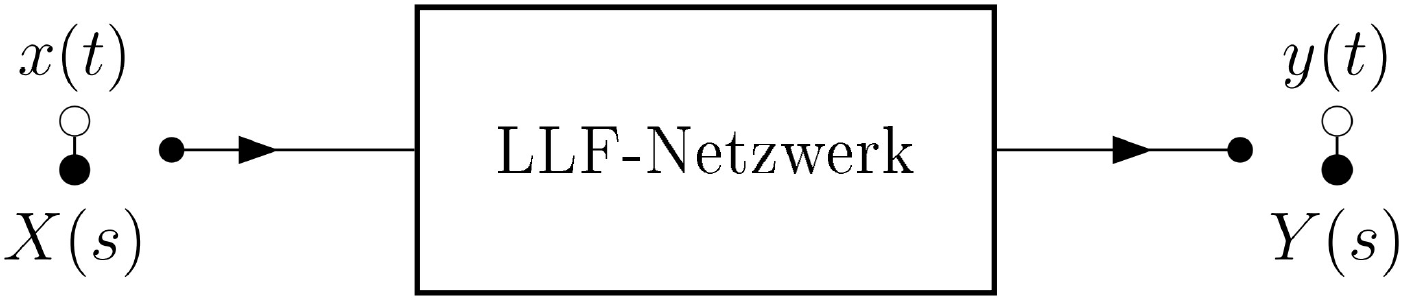
\includegraphics[width=\columnwidth]{images/llf_netzwerk.png}
\end{minipage}
\hfill
\begin{minipage}[c]{0.48\columnwidth}
    \raggedright% needed to suppress underfull hbox warning
    Die Betrachtungen beschränken sich auf \textbf{zeitinvariante} LLF-Netzwerke (lineare Netzwerke mit konzentrierten Elementen)
\end{minipage}


\subsection{Zusammenhang Frequenzgang -- UTF}{211}

Alle LTI-Systeme lassen sich mit einer Differntialgleichung der folgenden Form beschreiben:
$$ a_n \frac{\diff^n y}{\diff t^n} + a_{n-1} \frac{\diff^{n-1} y}{\diff t^{n-1}} + \cdots + a_1 \frac{\diff y}{\diff t} + a_0 y =
    b_m \frac{\diff^m x}{\diff t^m} + b_{m-1} \frac{\diff^{m-1} x}{\diff t^{m-1}} + \cdots + b_1 \frac{\diff x}{\diff t} + b_0 x  $$

Die Laplace-Transformierte der DGL hat die Form 
$$ \boxed{ H(s) = \frac{Y(s)}{X(s)} = \frac{b_m s^m + b_{m-1} s^{m-1} + \cdots + b_1 s + b_0}
{a_n s^n + a_{n-1} s^{n-1} + \cdots + a_1 s + a_0}  = \frac{N(s)}{D(s)} }$$

\begin{ctabular}{Ol}
    N(s) & Zählerpolynom mit konstanten, reellen Koeffizienten \\
    D(s) & Nennerpolynom mit konstanten, reellen Koeffizienten \\
    x(t) & Eingangssignal \\
    y(t) & Ausgangssignal \\
\end{ctabular}

\vspace{0.2cm}

Die Wurzeln der Gleichung $N(s) = 0$ ergeben $m$ endliche Nullstellen; die Wurzeln von $D(s) = 0$ ergeben $n$ Pole des Systems.
\textbf{Aus Stabilitätsgründen müssen alle Pole in der linken Halbebene (LHE) liegen!}


\subsubsection{Praktische Schreibweise für Pol-/Nullstellen}

Um die Pole bzw. Nullstellen des Systems direkt ablesen zu können, wird $H(s)$ faktorisiert. \textrightarrow\ Die UTF $H(s)$ ist durch
die Pole, Nullstellen und den Faktor $K$ \textbf{vollständig bestimmt}!

$$ H(s) = \underbrace{\frac{b_m}{a_m}}_{K} \cdot \frac{\prod\limits_{i=1}^m (s - z_i)}{\prod\limits_{j=1}^n (s - p_j)} $$


Da die Wurzeln von Polynomen mit reellen Koeffizienten entweder reell sind oder in konjugiert-komplexen Paare auftreten, ist es meistens
sinnvoll, die Systemfunktionen als Produkt von Faktoren 1. und 2. Ordnung mit reelen Koeffizienten darzustellen.

$$ H(s) = \underbrace{\frac{b_m}{a_m}}_{K} \cdot 
    \frac{\prod\limits_{i=1}^r (\cbl{s^2 + 2 \sigma_{zi} s + \omega_{zi}^2}) \prod\limits_{i=2r+1}^m (\cgn{s - z_i})}
    {\prod\limits_{j=1}^t (\cor{s^2 + 2 \sigma_{pj} s + \omega_{pj}^2}) \prod\limits_{j=2t+1}^n (\cvt{s - p_j})} $$

\textbf{Legende:}
\begin{itemize}
    \item \cbl{Beschreibt komplex-konjugierte Nullstellen in der LHE} 
    \item \cgn{Beschreibt reelle Nullstellen in der LHE}
    \item \cor{Beschreibt komplex-konjugierte Pole in der LHE} 
    \item \cvt{Beschreibt reelle Pole in der LHE} 
\end{itemize}

\vspace{0.2cm}

Alternativ kann $H(s)$ mittels \textbf{Polfrequenzen} und \textbf{Polgüten} beschrieben werden:
$$ H(s) = \underbrace{\frac{b_m}{a_m}}_{K} \cdot 
    \frac{\prod\limits_{i=1}^r (s^2 + \frac{\omega_{zi}}{q_{zi}} s + \omega_{zi}^2) \prod\limits_{i=2r+1}^m (s - z_i)}
    {\prod\limits_{j=1}^t (s^2 +\frac{\omega_{pj}}{q_{pj}} s + \omega_{pj}^2) \prod\limits_{j=2t+1}^n (s - p_j)} $$

\begin{ctabular}{Ol Ol}
    \omega_{pj}   & Polstellenfrequenzen  & \omega_{zi}   & Nullstellenfrequenzen \\
    q_{pj}        & Polstellengüten       & q_{zi}        & Nullstellengüten
\end{ctabular}


\subsection{Pol-/Nullstellendiagramme}{212}

\begin{minipage}[c]{0.35\columnwidth}
    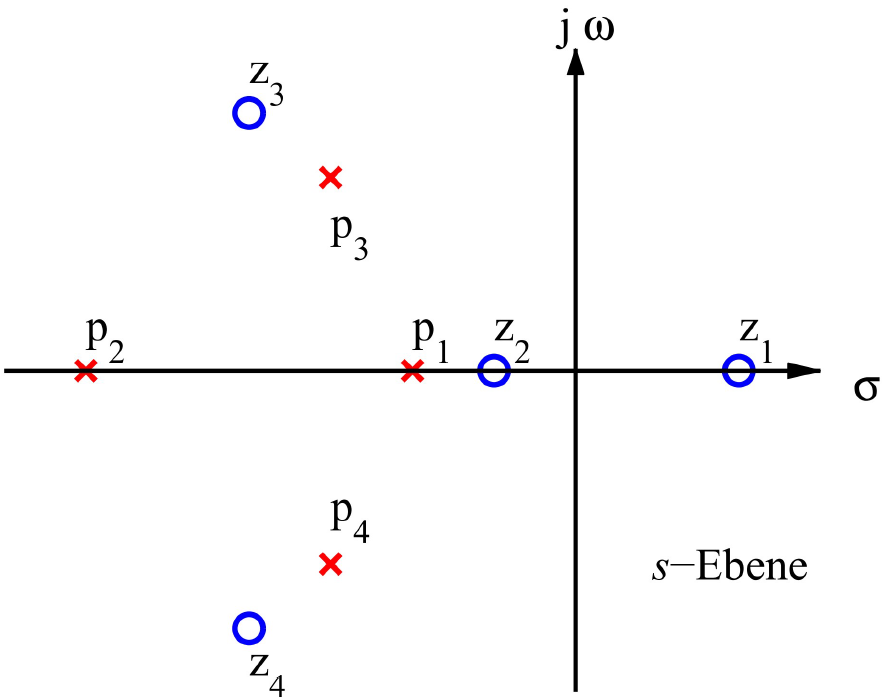
\includegraphics[width=\columnwidth]{images/pol_nullstellen_diagramm.png}
\end{minipage}
\hfill
\begin{minipage}[c]{0.63\columnwidth}
    Werden die Pole und Nullstellen in der komplexen Zahlenebene dargestellt, so spricht man von einem Pol-/Nullstellen-Diagramm.

    In Matlab erzeugt der Befehl \mylstbox{pzmap} einen solchen Plot

    \begin{tabular}{ll}
        Pole    & Kreuze \\
        NS      & Kreise \\
    \end{tabular}
\end{minipage}


\subsection{Stabilitätsbetrachtung im Pol-/Nullstellendiagramm}

Für \textbf{Grenzstabilität} gilt eine \textbf{UND-Verknüpfung} der aufgeführten Punkte. 
Für \textbf{Stabilität und Instabilität} gilt eine \textbf{ODER-Verknüpfung} der aufgeführten Punkte.

\begin{outline}
    \1 \textbf{Stabil:} 
        \2 Alle Polstellen in linker Halbebene (LHE)
        \2 Keine Polstellen vorhanden 
    \1 \textbf{Asymptotisch stabil:}
        \2 Polstellen nur in der linken Halbebene (LHE)
    \1 \textbf{Grenzstabil:} 
        \2 \textbf{Keine} Polstellen in der rechten Halbebene (RHE)
        \2 Mindestens eine \textbf{einfache Polstelle} auf imaginärer Achse
        \2 \textbf{Keine doppelten} Polstellen auf der imaginären Achse
    \1 \textbf{Instabil:} 
        \2 Mindestens eine Polstelle in der rechten Halbebene (RHE)
        \2 Mindestens eine \textbf{mehrfache Polstelle} auf der imaginären Achse
\end{outline}


\subsection{Pole in der komplexen Zahlenebene}{214}

\example{Polynom 2. Ordnung mit komplex-konjugierten Polen}

\begin{minipage}[c]{0.45\columnwidth}
    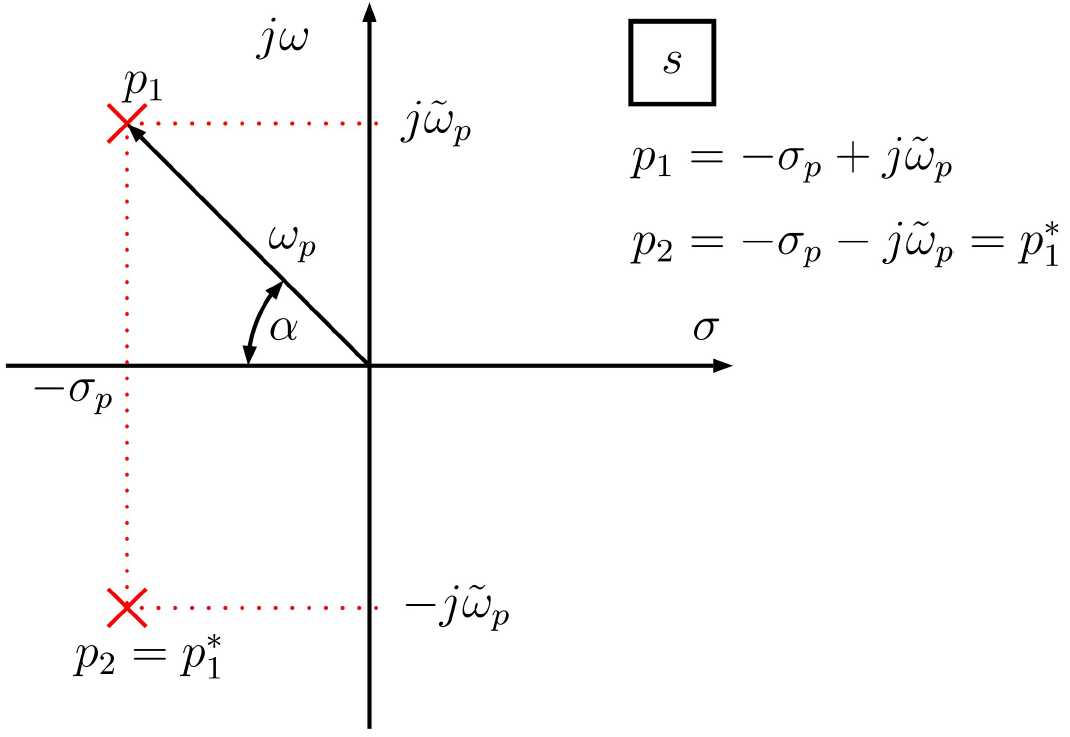
\includegraphics[width=\columnwidth]{images/beispiel_pol_nullstellen_diagramm.png}
\end{minipage}
\hfill
\begin{minipage}[c]{0.48\columnwidth}
    $$(s - p_1) \cdot (s -p_2) = s^2 + 2 \sigma_p s + (\sigma_p^2 + \tilde{\omega}_p^2) $$
    $$ \boxed{ \omega_p = \sqrt{\sigma_p^2 + \tilde{\omega}_p^2}} $$
    $$ \boxed{ q_p = \frac{\omega_p}{2 \sigma_p} = \frac{1}{2 \cdot \cos(\alpha)}} $$
\end{minipage}

\begin{tabular}{ll}
    $\omega_p$  & Polfrequenz \textrightarrow\ Entspricht Abstand des Pols vom Ursprung \\
    $q_p$       & Polgüte \\
\end{tabular}

\vspace{0.2cm}
\textbf{\myul{Grenzfälle}} \\
\begin{tabular}{lll}
    $\sigma_p = \omega_p$   & Doppelpol auf neg. reeller Achse  & \textrightarrow\ $q_p = \frac{1}{2}$ \\
    $\sigma_p = 0$          & Polpaar auf imaginärer Achse      & \textrightarrow\ $q_p = \infty$
\end{tabular}


\subsubsection{Reelle Pole}

\begin{minipage}[c]{0.48\columnwidth}
    $$ \boxed{ \omega_p = \sqrt{\sigma_{p1} \cdot \sigma_{p2} } } $$
\end{minipage}
\hfill
\begin{minipage}[c]{0.48\columnwidth}
    $$ \boxed{ q_p =  \frac{\sqrt{\sigma_{p1} \cdot \sigma_{p2}}}{\sigma_{p1} + \sigma_{p2}} \leq \frac{1}{2} } $$
\end{minipage}

\begin{itemize}
    \item[] \textrightarrow\ Für einzelne (reelle) Pole ist ist die Güte $q_p$ nicht definiert.
    \item[] \textrightarrow\ Die Polfrequenz $\omega_p$ entspricht dem Abstand zum Ursprung.
\end{itemize}

\textbf{\myul{Identische Werte}} \\
\begin{tabular}{c c c}
    $\sigma_{p1} = \sigma_{p2}$ & & $| q_p | = \frac{1}{2}$
\end{tabular}


\subsubsection{Verallgemeinerung des Beispiels}{214}

\begin{minipage}[c]{0.55\columnwidth}
    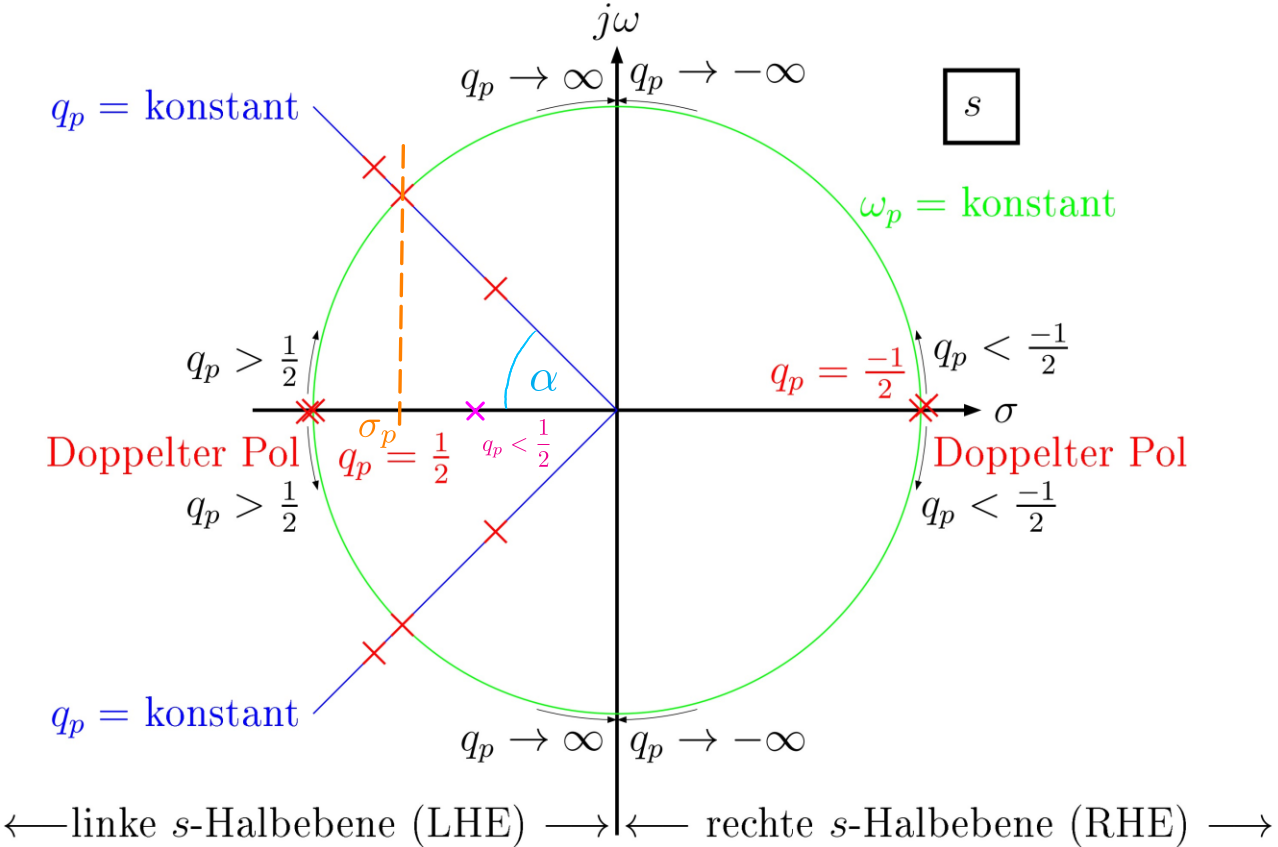
\includegraphics[width=\columnwidth]{images/pole_nullstellen_koeffizienten.png}
\end{minipage}
\hfill
\begin{minipage}[c]{0.42\columnwidth}
    \raggedright% needed to suppress underfull hbox warning
    \textbf{Hinweise}
    \begin{itemize}
        \item Pole sind als rote Kreuze dargestellt
        \item Für die NS (Nullstellenfrequenzen, Nullstellengüten) gelten die gleichen
            geometrischen Beziehungen wie für die Polstellen
    \end{itemize}
\end{minipage}


\subsection{Bestimmung Frequenzgang aus UTF}{216}

Um den Frequenzgang zu erhalten, kann $s = \jimg \omega$ eingesetzt werden.

$$ \boxed{ H(\jimg \omega) = H(s) \Big|_{s = \jimg \omega} = |H(\jimg \omega)| \cdot e^{\jimg \theta(\omega)} } $$

\begin{center}
    \begin{tabular}{ll c | c ll}
        $H(s)$                  & Übertragungsfunktion (UTF)    & & $|H(\jimg \omega)|$    & Amplitudengang \\
        $H(\jimg \omega)$       & Frequenzgang                  & & $\theta(\omega)$       & Phasengang
    \end{tabular}
\end{center}

Der Frequenzgang bzw. Amplitudengang und Phasengang werden folgendermassen dargestellt:

\begin{itemize}
    \item \textbf{Nyquist-Diagramm} \\
        $H(\jimg \omega)$ wird in Polarkoordinaten mit $\omega$ als Parameter aufgezeichnet 
    \item \textbf{Bode-Diagramm} \\
        $\alpha_{\deci \bel}(\omega)$ und $\theta(\omega)$ werden je in Funktion von $\log_{10}(\omega)$ aufgezeichnet
\end{itemize}


\subsection{Bestimmung Frequenzgang aus Pol-/Nullstellendiagramm}

Durch einsetzen einer beliebigen Auswertungsfrequenz $\jimg \omega_0$ in die Übertragungsfunktion $H(s)$ ergibt sich der
Frequenzgang $H(\jimg \omega_0)$ als:

$$ H(\jimg \omega_0) = K \cdot \frac{(\jimg \omega_0 - z_1) (\jimg \omega_0 - z_2) \cdots (\jimg \omega_0 - z_m)}
                                {(\jimg \omega_0 - p_1) (\jimg \omega_0 - p_2) \cdots (\jimg \omega_0 - p_n)}
                                = | H(\jimg \omega_0) | \cdot e^{\jimg \theta (\omega_0)} $$

Die einzelnen Faktoren in Zähler und Nenner können in Betrag und Phase aufgeteilt werden, beispielsweise folgendermassen:
$$ (\jimg \omega_0 - p_1) = |\jimg \omega_0 - z_1| \cdot e^{\jimg \theta_{z1}} = A_{z1} \cdot e^{\jimg \theta_{z1}} $$



Angewendet auf alle Faktoren kann der Frequenzgang $H(\jimg \omega_0)$ in den \cor{Amplitudengang $|H(\jimg \omega)|$} und den
\cgn{Phasengang $\theta(\omega)$} separiert werden:

$$ \boxed{ H(\jimg \omega_0) = K \cdot \frac{\cor{A_{z1} \cdot A_{z2} \cdots A_{zm}} \cdot \cgn{e^{\jimg(\theta_{z1} + \cdots + \theta_{zm})}}}
                                        {\cor{A_{p1} \cdot A_{p2} \cdots A_{pm}} \cdot \cgn{e^{\jimg(\theta_{p1} + \cdots + \theta_{pm})}}} } $$

\vspace{0.2cm}
\begin{minipage}[t]{0.48\columnwidth}
    \begin{center}
        \textbf{Betrag}
    \end{center}
    \vspace{-0.2cm}
    $$ \boxed{ | H(\jimg \omega_0) | = K \cdot \frac{\prod\limits_{i=1}^{m} A_{zi}}{\prod\limits_{j=1}^{n} A_{pj}} } $$
\end{minipage}
\hfill
\begin{minipage}[t]{0.48\columnwidth}
    \begin{center}
        \textbf{Phase}
    \end{center}
    \vspace{-0.2cm}
    $$ \boxed{ \theta(\omega_0) = \underbrace{\text{Phase von } K}_{\text{meistens } 0} + \sum_{i=1}^{m} \theta_{zi} - \sum_{j=1}^{m} \theta_{pj} } $$
\end{minipage}


\subsubsection{Zusammenhang mit Pol-/Nullstellendiagramm}

\begin{minipage}[c]{0.5\columnwidth}
    \begin{center}
    \begin{tikzpicture}
        [
            scale = 0.6,
            >=latex,
            ns/.style={circle, draw=blue, fill=white, thick, inner sep=0pt, minimum size=3pt},
            pol/.style={cross out, draw=red, inner sep=0pt, minimum size=3pt} 
        ]
        \begin{axis}
            [
                xmin=-4, xmax=2.5, ymin=-5, ymax=5, axis lines=middle,
                x label style={anchor=west},
                xlabel=$\sigma$,
                y label style={anchor=south},
                ylabel=$j \omega$,
                %grid
            ]
            
            % defines for arch
            \def\arrowRadius{5mm}                                           % radius of the circle that the arrow bends around

            % nodes
            \node[label=left: $j \omega_0$, inner sep = 0pt]       (freq0)     at (0, 1)       {};
            \draw                                                   (-0.05, 1) -- (0.05, 1);

            \node[label=left: $j \omega_1$, inner sep = 0pt]        (freq1)     at (0, 3)       {};
            \draw                                                   (-0.05, 3) -- (0.05, 3);

            \node[ns, label=left: $z_1$]                            (z1)        at (-3, 4)      {};
            \draw                                                   (z1) -- (-2, 4);
            \draw [-latex, green, semithick]                        (-2.5, 4) arc (0:330:\arrowRadius); %(start:end:radius)
            \node[label={[green]right:$\theta_{z1}$}]               (theta1)    at (-2.5, 4.3)    {};

            \node[ns, label=left: $z_2$]                            (z2)        at (-3, -4)     {};
            \draw                                                   (z2) -- (-2, -4);   
            \draw [-latex, green, semithick]                        (-2.5, -4) arc (0:45:\arrowRadius);
            \node[label={[green]right:$\theta_{z2}$}]               (theta2)    at (-2.6, -3.7)   {};

            \node[pol, label=below right: $p_1$]                    (p1)        at (1, 2)      {};
            \draw                                                   (p1) -- (2, 2); 
            \draw [-latex, green, semithick]                        (1.5, 2) arc (0:205:\arrowRadius);
            \node[label={[green]right:$\theta_{p1}$}]               (theta3)    at (1.5, 2.3)    {};

            \node[pol, label=below: $p_2$]                          (p2)        at (1, -2)     {};
            \draw                                                   (p2) -- (2, -2); 
            \draw [-latex, green, semithick]                        (1.5, -2) arc (0:125:\arrowRadius);
            \node[label={[green]right:$\theta_{p2}$}]               (theta4)    at (1.5, -1.7)    {};

            
            \draw[thick, orange]        (freq0) to node[above]      {$A_{z1}$}  (z1);
            \draw[thick, orange]        (freq0) to node[below]      {$A_{z2}$}  (z2);
            \draw[thick, orange]        (freq0) to node[below right]{$A_{p1}$}  (p1);
            \draw[thick, orange]        (freq0) to node[below left] {$A_{p2}$}  (p2);
           
        \end{axis}
        
    \end{tikzpicture}
\end{center}

    % Hier mit nur einer Nullstelle (keine Pole): 
    % 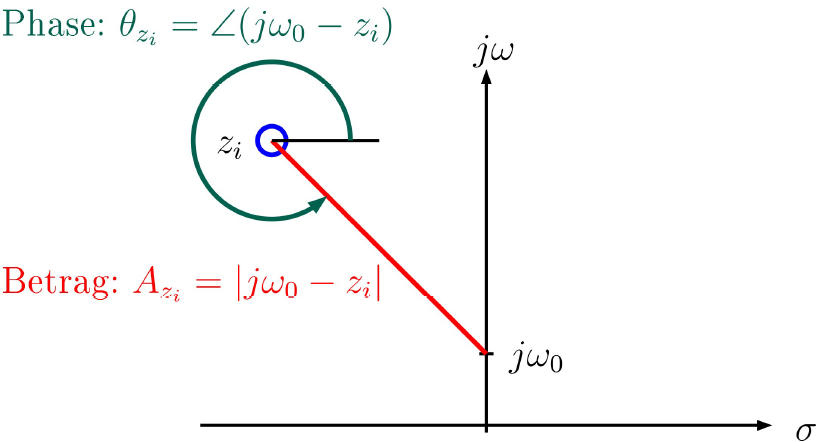
\includegraphics[width=\columnwidth]{images/frequenzgang_amplitudengang.png}
\end{minipage}
\hfill
\begin{minipage}[c]{0.48\columnwidth}
    Die Auswertungsfrequenz $\jimg \omega$ ist variabel und 'wandert' auf der \textbf{imaginären Achse}.
    Für eine bestimmte Auswertungsfrequenz $\jimg \omega_0$ können die Faktoren von $H(\jimg \omega_0)$ als \cor{Abstand}
    und \cgn{Phase} zu den Pol- bzw Nullstellen interpretiert werden.
    Somit kann grafisch aus dem Pol-/Nullstellendiagramm ein Rückschluss auf den Amplitudengang gezogen werden.
    $$ H(\jimg \omega_0) = K \cdot \frac{\cor{A_{z1} \cdot A_{z2}} \cdot \cgn{e^{\jimg(\theta_{z1} + \theta_{z2})}}}
    {\cor{A_{p1} \cdot A_{p2}} \cdot \cgn{e^{\jimg(\theta_{p1} + \theta_{p2})}}}  $$
\end{minipage}


% \subsubsection{Rückschlüsse auf Amplitudengang}

% \begin{outline}
%     \1 Es werden vor allem die \textbf{Abstände} betrachtet 
%     \1 Pol- und Nullstellen können sich aufheben
%     \1 Bei $\omega = 0$ gilt:
%         \2 Wenn Nullstelle \textrightarrow\ $|H(\jimg \omega_0)| = \infty$ \textrightarrow\ $\theta(\jimg \omega_0) = \frac{\pi}{2}$
%         \2 Wenn Pol \textrightarrow\ $|H(\jimg \omega_0)| = 0$ \textrightarrow\ $\theta(\jimg \omega_0) = -\frac{\pi}{2}$
%         \2 Wenn weder Pol noch NS \textrightarrow\ $|H(\jimg \omega_0)|$ hat endlichen Wert \textrightarrow\ $\theta(\jimg \omega_0) = 0$
%     \1 Bei $\omega = \infty$ gilt:
%         \2 Wenn Zählergrad $>$ Nennergrad \textrightarrow\ $|H(\jimg \omega_0)| = \infty$
%         \2 Wenn Zählergrad $=$ Nennergrad \textrightarrow\ $|H(\jimg \omega_0)|$ hat endlichen Wert
%         \2 Wenn Zählergrad $<$ Nennergrad \textrightarrow\ $|H(\jimg \omega_0)| = 0$
% \end{outline}


\subsection{Vorgehen Frequenzgang aus Pol-NS-Diagramm ermitteln}

\begin{itemize}
    \item $(\text{Schluss-Steigung } = \text{ Anzahl Nullstellen } - \text{ Anzahl Polstellen}) \cdot 20 \, \deci \bel / \Dek$
    \item Sind im Ursprung \textbf{keine} Pole / Nullstellen, so ist die Steigung für tiefe Frequenzen $= 0$
    \item Befinden sich am gleichen Ort eine Polstelle \textbf{und} eine Nullstelle, so heben sie sich auf
    \item Einfache reelle Nullstelle: Ab dieser Frequenz Steigung von  $+20 \, \deci \bel / \Dek$
    \item Einfacher reeler Pol: Ab dieser Frequenz Steigung von  $-20 \, \deci \bel / \Dek$
    \item Sind im Pol-NS-Diagramm komplex-konjugierte Polstellen vorhanden, so enthält der Amplitudengang \textbf{Überschwinger}
    \item Sind im Pol-NS-Diagramm komplex-konjugierte Nullstellen vorhanden, so enthält der Amplitudengang \textbf{Senken}
    \item Pole bzw. Nullstellen mit \textbf{kleinstem Abstand} zum Ursprung haben am meisten Einfluss
\end{itemize}


\subsection{Allpassnetzwerk}{220}

Ein Allpass ist ein Netzwerk, bei dem der \textbf{Amplitudengang für alle Kreisfrequenzen $\bm{\omega}$ konstant} ist
$$ \boxed{\abs{H(\jimg \omega)} = \const \neq 0}$$

\textrightarrow\ Im Pol-/Nullstellendiagramm ist ein Allpass dargestellt durch eine 
\textbf{zur $\bm{\jimg \omega}$-Achse symmetrische Pol-/Nullstellenkonfiguration}

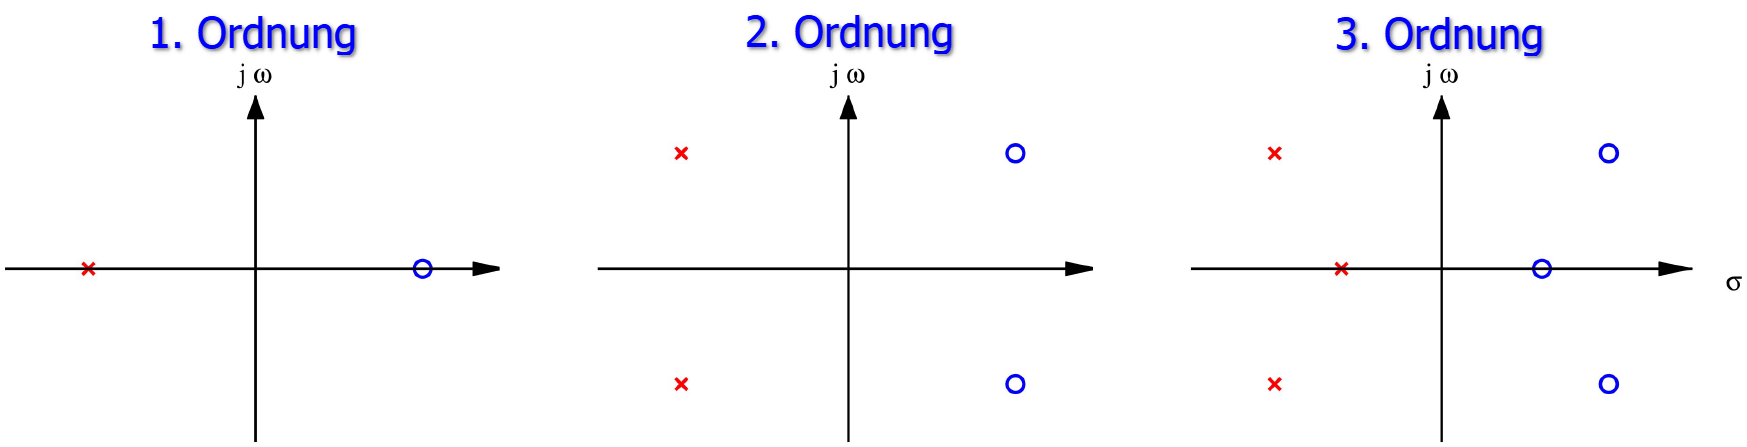
\includegraphics[width=\columnwidth]{images/allpass.png}

$$ \boxed{ \text{UTF Allpass: } H_A(s) = K \cdot \frac{Q(-s)}{Q(s)} } $$

Für einen Allpass gilt:
\begin{itemize}
    \item Ein stabiler Allpass besitzt einen \textbf{streng monoton abfallenden} Phasengang
    \item Jede beliebige (realisierbare) UTF $H(S)$ kann \textbf{immer} in ein allpassfreies Netzwerk $H_M(s)$ und einen Allpass $H_A(s)$
        \textbf{zerlegt} werden (\textrightarrow\ siehe Beispiel Abschnitt ~\ref{Beispiel Zerlegung})
        $$ \boxed{ H(s) = H_M(s) \cdot H_A(s) }$$
\end{itemize}


\subsection{Minimalphasige- und nicht-minimalphasige Systeme}{221}

\begin{outline}
    \1 Minimalphasennetzwerke: 
        \2 besitzen \textbf{keine Nullstellen in der rechten Halbebene (RHE)}
        \2 \textbf{entweder} ein frei wählbarer Amplituden- \textbf{oder} Phasengang
    \1 Nicht-Minimalphasennetzwerke
        \2 Amplituden- und Phasengang unabhängig voneinander wählbar
\end{outline}


\example{Zerlegung nicht-minimalphasiges System}
\label{Beispiel Zerlegung}

Ein nicht-minimalphasiges System kann in ein minimalphasiges System und einen Allpass zerlegt werden
(\textrightarrow\ \textbf{Multiplikation!}). 

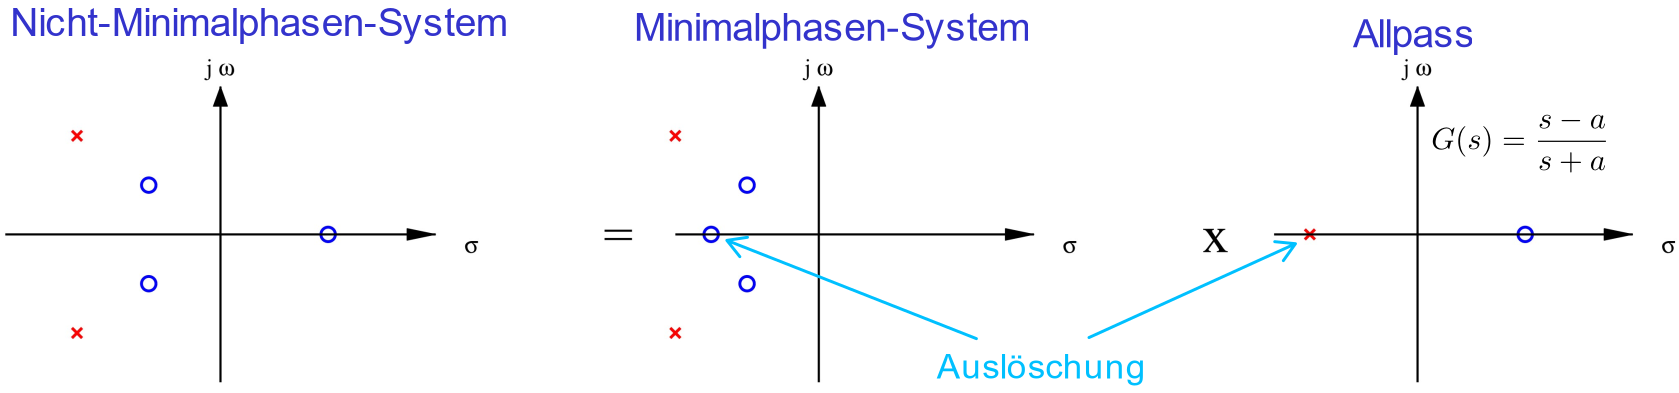
\includegraphics[width=\columnwidth]{images/beispiel_minimalphasensystem.png}



